\documentclass{article}

\usepackage[a4paper, total={6in, 9in}]{geometry}
\usepackage[utf8]{inputenc}
\usepackage{graphicx}
\usepackage{accents}
\usepackage[colorlinks=true,urlcolor=blue]{hyperref}

\title{Relazione progetto Calcolo numerico\\Appello straordinario per laureandi Febbraio-Aprile 2023\\Laurea in Informatica}
\date{22 Febbario 2023}
\author{Luca Busacca - 1227589}
\makeindex

\begin{document}
\maketitle
\vfill

{\hypersetup{linkcolor=black}
\renewcommand\contentsname{Indice}
\tableofcontents
}
\hfill
{\hypersetup{linkcolor=black}
\renewcommand{\listfigurename}{Elenco delle figure}
\listoffigures
}

\clearpage

\section{Introduzione}
Lo scopo del progetto è quello di stimare la soluzione del problema di ottimizzazione:
\[x^{*} = argmin_{x\in[a,b]}{f(x)}\]
In altre parole si vuole trovare il valore di x tale per cui vale che $f(x) = min(y)$.\\\\
A tale fine è stato fornito un set di dati contenente i valori di x e y tali che: $y_{i} = f(x_{i})+\epsilon$, ovvero dati affetti da rumore.\\\\
La richiesta è quella di costruire un modello surrogato $\widetilde f_{\alpha}(x)$ tale che:
\[x^{*}_{\alpha}=argmin_{x\in[a,b]}{\widetilde f_{\alpha}(x)}\]
Il problema viene affrontato cercando gli zeri della derivata della funzione mediante il metodo di Newton. La costruzione del modello surrogato risulta necessaria in quanto i dati affetti da rumore possono cambiare, e anche di molto, il valore del minimo.\\
Per la costruzione di tale modello vengono utilizzate tecniche di interpolazione polinomiale ed un approccio ai minimi quadrati con regolarizzazione alla Tikonov.\\\\
Per un'idea più dettagliata del problema che stiamo affrontando risulta conveniente effettuare un plot del dataset di partenza fissato:
\begin{figure}[h]
    \centering
    \label{fig:startinDataSet}
    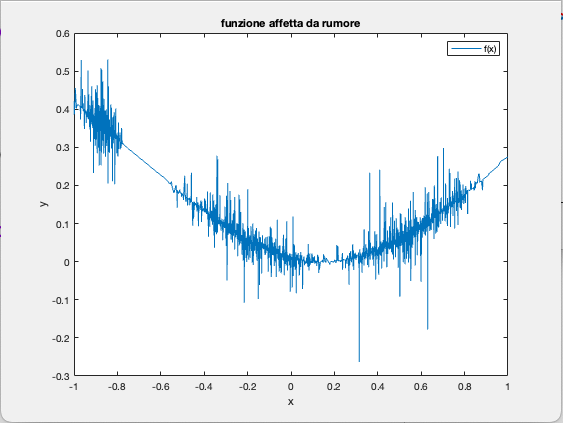
\includegraphics[width=1\textwidth]{images/funzione.png}
    \caption{Plot del dataset di partenza}
\end{figure}

\clearpage

\section{Svolgimento}
Dopo aver letto e compreso la consegna si è proceduto all'implementazione delle funzioni e dello script richiesto.\\\\
Per iniziare è stato scritto l'help della funzione \textbf{ChebDiff1D} che calcola la matrice di derivazione D della base di Chebyshev di grado n. Tale matrice ci permette di di calcolare la derivata di una funzione nella base di Chebyshev. L'unico parametro in input è il parametro \texttt{N} := grado della base di Chebyshev. L'output è la matrice \texttt{D} di dimensione [N+1 x N+1] calcolata dalla funzione.\\\\
Come secondo passo è stata implementata la funzione \textbf{cheb\_vand} che calcola la matrice di Vandermonde V della base di Chebyshev di grado n sui punti x. La funzione prende in input i parametri \texttt{n} := grado massimo di approssimazione del polinomio, e \texttt{x} := vettore colonna di punti compresi nell'intervallo [-1,1]. L'output restituito è la matrice di V di dimensione [N+1 x N+1] calcolata come segue:
\[V := cos(acos(x))*[0,1,\dots,n]\]\\
Successivamente si è proceduto a scrivere la funzione \textbf{cheb\_quad} che calcola il vettore colonna \texttt{xquad} degli n+1 nodi di Chebyshev-Lobatto nell'intervallo [-1,1], ed il vettori riga \texttt{w} degli n+1 pesi calcolato risolvendo il sistema dei momenti
\[(V^{quad})^{t}w=m\]
La funzione prevede in input il parametro \texttt{n} := grado di esattezza polinomiale. L'output della funzione corrisponde ai vettori \texttt{xquad} e \texttt{w} sopracitati.\\
All'interno della stessa viene fatto uso della funzione \textbf{cheb\_vand} precedentemente citata per il calcolo della matrice Vquad necessaria alla risoluzione del sistema lineare.\\
Per la risoluzione del sistema lineare vengono usate la tecnica di fattorizzazione LU con pivoting parziale e gli algoritmi di sostituzione avanti e indietro.\\\\
In seguito è stata creata la funzione \textbf{cheb\_tikonov} capace di trovare l'unico minimizzatore della funzione \texttt{cstar}, corrispondente alla soluzione del sistema lineare 
\[Gc=b\]
dove:
\[G=\frac{V^{t}V}{M}+\lambda G_{1}\]
\[b=\frac{V^{t}y}{M}\]
A seguito di una serie di osservazioni nel documento dell'esame è stata resa nota la matrice L ed è stato evidenziato che, se è nota tale matrice L tale per cui vale che
\[G=R0^{t}R0\]
dove R0 è la parte superiore quadrata della matrice R ottenuta mediante fattorizzazione QR di L, allora risolvere il sistema lineare equivale a risolvere
\[R0^{t}R0c=b\]
facilmente risolvibile mediante gli algoritmi di sostituzione avanti e indietro.\\
La funzione prende in input i parametri \texttt{n} := grado polinomiale, \texttt{lambda} := parametro di regolarizzazione alla Tikonov, \texttt{xsample} := vettore colonna dei punti di campionamento, \texttt{ysample} := vettore colonna dei valori di f(xsample) affetti da rumore.\\
La funzione restituisce in output il vettore colonna \texttt{cstar} di n+1 elementi precedentemente menzionato, la matrice \texttt{Rzero} di dimensioni [n+1 x n+1] calcolata come fattorizzazione di Cholesky di G ed il vettore colonna \texttt{b} di n+1 elementi corrispondente al termine noto del sistema.\\
All'interno della funzione vengono richiamate le funzioni \textbf{cheb\_vand} e \textbf{cheb\_quad} utili al calcolo degli elementi necessari a trovare la matrice L.\\
Come precedentemente anticipato si fa uso della funzione \texttt{qr} per calcolare la fattorizzazione QR della matrice L e delle funzioni di sostituzione avanti e indietro per la risoluzione del sistema lineare.\\\\
Infine è stato scritto uno script in cui, dopo aver caricato il dataset e definito le variabili necessarie al corretto funzionamento, è stata calcolata la matrice \texttt{D} per mezzo della function \textbf{ChebDiff1D} ed il vettore \texttt{cstar} per mezzo della function \textbf{cheb\_tikonov} e grazie a tali dati è stato possibile costruire il modello surrogato e le sue derivate prima e seconda. Successivamente grazie al metodo di Newton è stato possibile trovare il punto di minimo, obbiettivo del progetto.\\\\
È bene precisare che è stato necessario scegliere un punto da cui far partire il metodo di Newton e che per la scelta è stato utile osservare il grafico della derivata del modello surrogato:
\begin{figure}[!h]
    \centering
    \label{fig:derivata}
    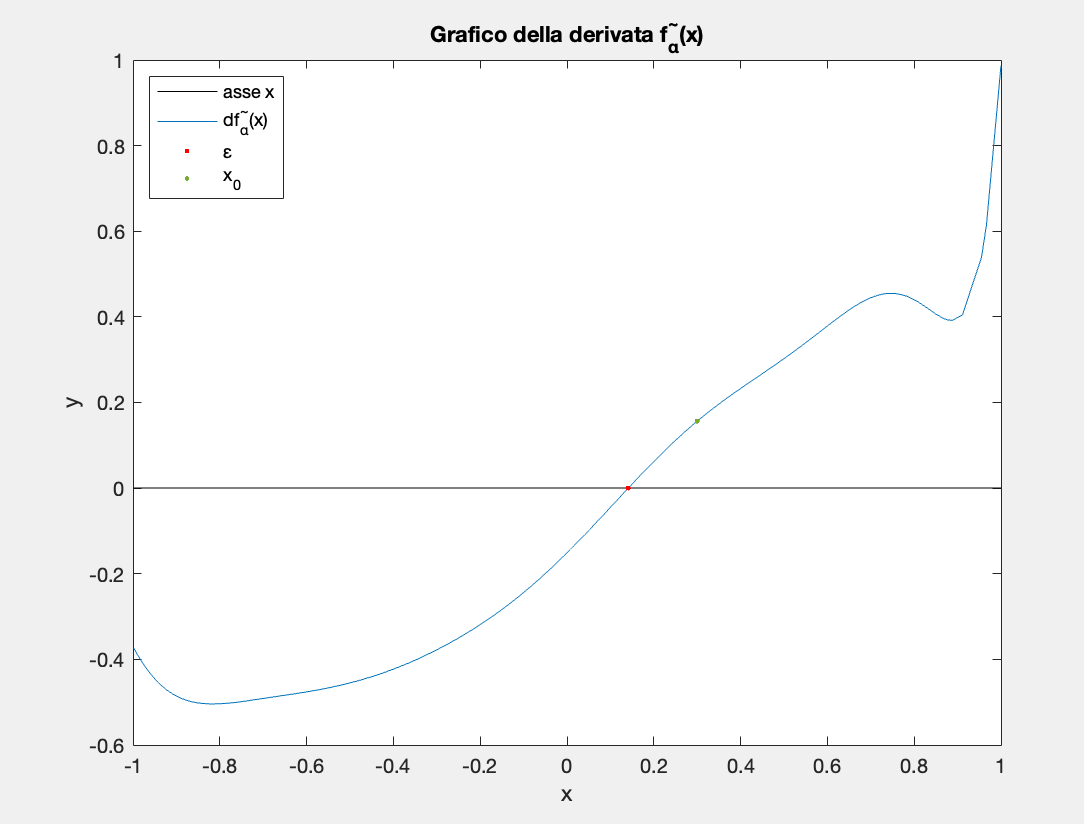
\includegraphics[width=1\textwidth]{images/derivata.png}
    \caption{Derivata del modello surrogato}
\end{figure}
\\Il punto di inizio considerato per il metodo di Newton è x = 0.3 .\\
\subsection*{Disclaimer}
Tutte le funzioni che sono state utilizzate e non son presenti all'interno della cartella come m files, sono supportare da R2022b. Per essere certo di ciò è stato eseguito un controllo al seguente link:
\begin{center}
    \url{https://it.mathworks.com/help/matlab/referencelist.html?type=function&listtype=alpha&category=index&blocktype=&capability=&s_tid=CRUX_lftnav}
\end{center}

\clearpage

\section{Conclusioni}
Grazie alla costruzione del modello surrogato è stato possibile utilizzare il metodo di Newton sulla funzione interpolante così da trovare il valore di x in cui tale modello assume il minimo.\\
Al fine di garantire il corretto funzionamento dell'algoritmo risulta necessario che i dati si trovino nell'intervallo [-1,1] e che rispettino le ipotesi del metodo di Newton.\\\\
Lanciando lo script è possibile osservare i seguenti risultati:
\begin{figure}[!h]
    \centering
    \label{fig:result}
    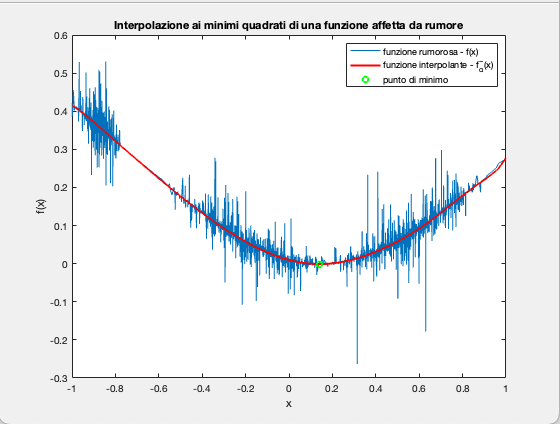
\includegraphics[width=1\textwidth]{images/risultato_figura.png}
    \caption{Grafico della funzione f(x) e del modello surrogato con punto di minimo trovato mediante Newton}
\end{figure}
\textbf{}\\\\
\begin{figure}[!h]
    \centering
    \label{fig:consoleResult}
    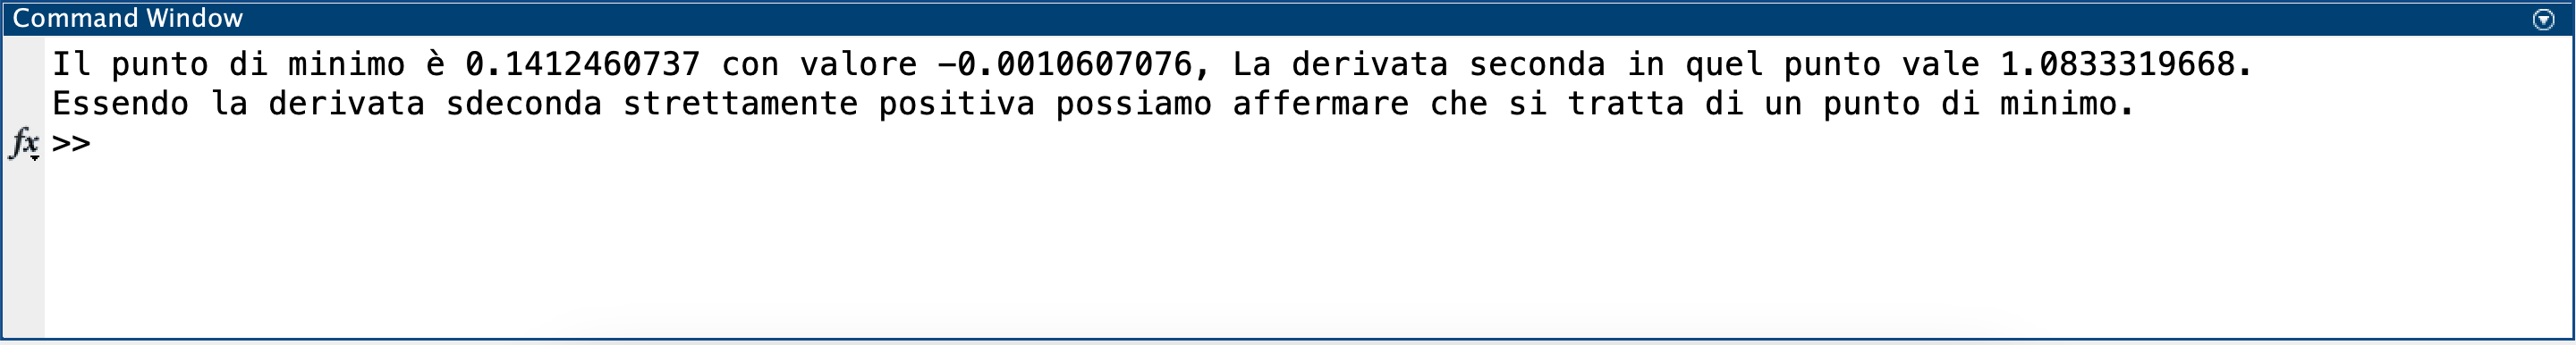
\includegraphics[width=1\textwidth]{images/risultato_console.png}
    \caption{Stampa dei risultati ottenuti in console}
\end{figure}
\end{document}